\documentclass[conference]{IEEEtran}
\IEEEoverridecommandlockouts
% The preceding line is only needed to identify funding in the first footnote. If that is unneeded, please comment it out.
% Template version as of 6/27/2024

\usepackage{cite}
\usepackage{amsmath,amssymb,amsfonts}
\usepackage{algorithmic}
\usepackage{graphicx}
\usepackage{textcomp}
\usepackage{xcolor}
\usepackage{booktabs}
\usepackage{multirow}
\usepackage{hyperref}

\def\BibTeX{{\rm B\kern-.05em{\sc i\kern-.025em b}\kern-.08em
    T\kern-.1667em\lower.7ex\hbox{E}\kern-.125emX}}

\begin{document}

\title{Consistency-Constrained Multi-Task Bengali Hate Speech Detection with Generative Explanations\\
}

\author{\IEEEauthorblockN{1\textsuperscript{st} Author A}
\IEEEauthorblockA{\textit{Department of Computer Science \& Engineering} \\
\textit{Affiliation Withheld for Peer Review}\\
City, Country \\
author.a@example.com}
\and
\IEEEauthorblockN{2\textsuperscript{nd} Author B}
\IEEEauthorblockA{\textit{Department of Computer Science \& Engineering} \\
\textit{Affiliation Withheld for Peer Review}\\
City, Country \\
author.b@example.com}
}

\maketitle

\begin{abstract}
Automated hate speech detection is predominantly framed as an isolated, single-task classification problem, ignoring the intrinsic hierarchical dependencies that link hate category, targeted demographic, and threat severity. In low-resource languages like Bengali, general-purpose Large Language Models (LLMs) struggle to preserve this logical consistency during generation, frequently outputting severe structural contradictions (e.g., classifying a comment as non-hateful while simultaneously asserting that an organization is targeted with severe intensity). In this paper, we propose an end-to-end Consistency-Constrained Multi-Task Learning (MTL) architecture based on BanglaBERT that jointly predicts Hate Type (5 classes), Target (5 classes), and Severity (3 classes). To mathematically enforce cross-task dependencies, we introduce a novel, fully differentiable Soft Consistency Loss that penalizes contradictory probabilistic states during backpropagation. Furthermore, to provide transparent accountability for content moderation, our model integrates a lightweight generative rationale decoder trained via knowledge distillation on 2,000 curated, human-audited Bengali explanations, producing natural language rationales alongside classifications. Rigorously evaluated on a strictly held-out test set of 3,553 Bengali comments (drawn from a 35,530-sample corpus), our 110M parameter model reduces the Consistency Violation Rate (CVR) from 9.46 percent (336 violations) in the unconstrained baseline to 0.03 percent (a single borderline violation), while simultaneously boosting Average Macro F1 from 0.540 to 0.558. In extensive benchmarking against dedicated Bengali LLMs---including TigerLLM-1B, TituLLM-1B, and BongLLaMA-3B under both zero-shot and 5-shot paradigms---our model achieves a 68.8 percent relative Macro F1 improvement over the strongest LLM baseline (0.558 vs. 0.330), operates approximately 390 times faster (0.0152s vs. 5.851s per sample), and guarantees 100 percent deterministic output parsing. Rationale faithfulness evaluated under the ERASER benchmark demonstrates a 22.6 percent gain in Area Over Perturbation Curve (AOPC), proving that task-specific architectural inductive bias significantly outperforms raw model scale for multi-aspect toxicity moderation in low-resource settings.
\end{abstract}

\begin{IEEEkeywords}
Bengali Hate Speech, Multi-Task Learning, Consistency Loss, Large Language Models, Explainable AI, Low-Resource NLP
\end{IEEEkeywords}

\section{Introduction}
Online social platforms across the Bengali-speaking world have experienced an unprecedented escalation in hate speech, communal vilification, and cyberbullying \cite{islam2021bangla, romim2022bdshs}. Automatic moderation is vital to safeguard digital spaces; however, Bengali presents distinct computational challenges due to complex agglutinative morphology, frequent phonetic transliteration (Banglish), widespread code-mixing, and subtle cultural nuances \cite{romero2019bengali, sazzed2021vulgarity}.

Conventional NLP frameworks predominantly treat hate speech detection as an isolated binary (toxic vs. non-toxic) or multi-class classification problem \cite{romero2021hate, karim2020deephateexplainer}. While adequate for basic keyword filtering, this disjoint formulation ignores the multi-dimensional anatomy of online toxicity: identifying \textit{what} category of hate is manifested (Type), \textit{who} is being attacked (Target), and \textit{how severe} the threat is (Severity). Crucially, these dimensions are governed by strict semantic dependencies:
\begin{equation}
\text{Type} = \text{None} \iff \text{Target} = \text{None} \land \text{Severity} = \text{Little to None}
\label{eq:semantic_rule}
\end{equation}
If a comment is non-hateful, it logically cannot target an entity nor inflict severe harm. Standard multi-task classifiers and generative Large Language Models (LLMs) routinely violate this semantic hierarchy, generating glaring hallucinations that compromise automated moderation pipelines.

Recently, generative LLMs such as LLaMA \cite{touvron2023llama} and regionally fine-tuned models like TigerLLM \cite{nishat2025tigerllm, raihan2025tigerllm} have demonstrated impressive general reasoning. However, as our empirical experiments demonstrate, applying LLMs to multi-aspect classification in low-resource languages reveals three critical failure modes:
\begin{enumerate}
    \item \textbf{Structural Hallucinations \& Mode Collapse:} Unconstrained LLMs frequently produce incompatible attribute combinations (e.g., TigerLLM outputs 47 consistency violations, while BongLLaMA-3B suffers catastrophic mode collapse with 100\% violations under few-shot prompting).
    \item \textbf{Syntax and Format Fragility:} Prompting LLMs for structured JSON outputs is highly brittle; without extensive demonstrations, foundation models like TituLLM and BongLLaMA exhibit format failure rates between 78.5\% and 100\%.
    \item \textbf{Prohibitive Operational Latency:} Evaluating 1B--3B parameter LLMs incurs inference latencies between 1.28s and 5.85s per comment, rendering them computationally unusable for real-time edge moderation streams handling millions of daily posts.
\end{enumerate}

To resolve these challenges, we present a unified, efficient, and interpretable framework for Bengali hate speech detection. Our main contributions are:
\begin{itemize}
    \item \textbf{Consistency-Constrained Multi-Task Architecture:} We formulate multi-aspect Bengali hate speech detection as a joint optimization problem over BanglaBERT \cite{bhattacharjee2022banglabert}, simultaneously predicting Hate Type (5 classes), Target (5 classes), and Severity (3 classes).
    \item \textbf{Differentiable Soft Consistency Loss:} We propose a novel loss term $\mathcal{L}_{\text{consist}}$ that mathematically penalizes contradictory probability mass during backpropagation, reducing consistency violations from 9.46\% (336 violations) to 0.03\% (1 violation) while acting as an inductive regularizer that boosts overall Macro F1 by +3.3\%.
    \item \textbf{Dual-Layer Explainability via Rationale Distillation:} We bridge extractive feature attribution (evaluated via ERASER metrics \cite{deyoung2020eraser}) and generative natural language explanations by training a lightweight LSTM decoder on 2,000 curated, human-audited Bengali rationales distilled from a frontier teacher model \cite{team2023gemini}.
    \item \textbf{Rigorous Benchmark Against Bengali LLMs:} We establish the first standardized benchmark comparing specialized small language models (SLMs) against dedicated Bengali LLMs (TigerLLM-1B, TituLLM-1B, BongLLaMA-3B) under both zero-shot and 5-shot paradigms on an identical held-out test set of 3,553 samples.
\end{itemize}

\section{Related Work}
\label{sec:related}

\subsection{Bengali Hate Speech Detection}
Early Bengali hate speech detection relied primarily on n-gram feature extraction, Support Vector Machines, and recurrent networks \cite{romero2019bengali, islam2021bangla}. Subsequent benchmark initiatives introduced larger collections such as BD-SHS \cite{romim2022bdshs} and investigations into transliterated vulgarity \cite{sazzed2021vulgarity}. The introduction of transformer models, specifically BanglaBERT \cite{bhattacharjee2022banglabert}, advanced Bengali NLP by pretraining an ELECTRA discriminator architecture \cite{clark2020electra} over 16.5 GB of curated Bengali web corpora. While recent multi-aspect datasets such as BanglaMultiHate \cite{hasan2026banglamultihate, hasan2023banglamultihate} introduced multi-dimensional annotations, existing approaches treat these dimensions as isolated classification targets, failing to enforce cross-task logical constraints.

\subsection{Multi-Task Learning and Constraint Enforcement}
Multi-Task Learning (MTL) enhances feature generalization by sharing hidden representations across related prediction objectives \cite{caruana1997multitask, liu2019mt}. However, hard parameter sharing does not inherently prevent separate classification heads from outputting mutually contradictory decisions. While post-hoc rule-based heuristics can overwrite invalid combinations during inference, they do not provide gradient feedback to guide the encoder's internal representations during training. Our framework directly embeds taxonomic dependencies into the loss function via a differentiable penalty.

\subsection{Explainable AI (XAI) in Low-Resource NLP}
Model interpretability is essential for accountability in automated content moderation \cite{deyoung2020eraser}. While post-hoc token attribution techniques like LIME \cite{ribeiro2016why} have been adapted to detect arrogant and abusive Bengali comments \cite{ashraf2026arrogant, karim2020deephateexplainer}, feature attribution heatmaps do not provide human-readable textual justifications. Meanwhile, evaluating frontier LLMs in multilingual and low-resource environments has documented significant performance degradation compared to English benchmarks \cite{ahuja2023mega}. We bridge these gaps by combining extractive token evaluation with generative natural language rationales.

\section{Methodology}
\label{sec:method}

\subsection{Task Definition and Structural Hierarchy}
Given an input Bengali text sequence $X = (x_1, x_2, \dots, x_L)$, our objective is to jointly predict a classification tuple $\hat{\mathbf{y}} = (\hat{y}^{\text{type}}, \hat{y}^{\text{target}}, \hat{y}^{\text{sev}})$ and generate an explanatory text sequence $\hat{E} = (\hat{e}_1, \dots, \hat{e}_M)$. The label spaces are defined as:
\begin{itemize}
    \item $\mathcal{Y}^{\text{type}} = \{\text{None}, \text{Abusive}, \text{Political Hate}, \text{Religious Hate}, \text{Gender Hate}\}$ ($K_1 = 5$)
    \item $\mathcal{Y}^{\text{target}} = \{\text{None}, \text{Individual}, \text{Organization}, \text{Community}, \text{Society}\}$ ($K_2 = 5$)
    \item $\mathcal{Y}^{\text{sev}} = \{\text{Little to None}, \text{Mild}, \text{Severe}\}$ ($K_3 = 3$)
\end{itemize}

The taxonomy enforces the structural constraint in \eqref{eq:semantic_rule}. Any output where $\hat{y}^{\text{type}} = \text{None}$ but $\hat{y}^{\text{target}} \neq \text{None}$ or $\hat{y}^{\text{sev}} \neq \text{Little to None}$ constitutes a severe consistency violation.

\subsection{Model Architecture}
Our architecture consists of three integrated components:
\begin{enumerate}
    \item \textbf{Shared Transformer Encoder:} We utilize pretrained BanglaBERT \cite{bhattacharjee2022banglabert} ($d = 768$, 110M parameters). Given token sequence $X$, the encoder produces contextual representations $\mathbf{H} = \text{BanglaBERT}(X) \in \mathbb{R}^{L \times d}$. The pooled representation $\mathbf{h}_{\text{CLS}} = \mathbf{H}_0 \in \mathbb{R}^d$ captures global sequence semantics.
    
    \item \textbf{Multi-Task Classification Heads:} The representation $\mathbf{h}_{\text{CLS}}$ is routed into three parallel two-layer MLPs with ReLU activation and dropout ($p = 0.3$):
    \begin{equation}
    \hat{\mathbf{y}}^t = \text{Softmax}\left(\mathbf{W}_2^t \text{ReLU}(\mathbf{W}_1^t \mathbf{h}_{\text{CLS}} + \mathbf{b}_1^t) + \mathbf{b}_2^t\right)
    \end{equation}
    for $t \in \{\text{type}, \text{target}, \text{sev}\}$.
    
    \item \textbf{Autoregressive Rationale Decoder:} To provide interpretable explanations, we incorporate an LSTM decoder ($d_{\text{embed}} = 256$, $d_{\text{hidden}} = 512$). Initial hidden and cell states are projected directly from $\mathbf{h}_{\text{CLS}}$:
    \begin{equation}
    \mathbf{h}_0 = \tanh(\mathbf{W}_h \mathbf{h}_{\text{CLS}}), \quad \mathbf{c}_0 = \tanh(\mathbf{W}_c \mathbf{h}_{\text{CLS}})
    \end{equation}
    During training, the decoder is trained via teacher forcing to generate natural language explanations token-by-token.
\end{enumerate}

\subsection{Loss Formulation}
To counteract extreme class imbalance (e.g., Gender Hate comprises $<1\%$ of the dataset), we employ multi-class Focal Loss \cite{lin2017focal} across all three heads:
\begin{equation}
\mathcal{L}_{\text{focal}}^t = -\frac{1}{N} \sum_{i=1}^N \alpha_{y_i^t} (1 - P(y_i^t | X_i))^\gamma \log P(y_i^t | X_i)
\end{equation}
where $\gamma = 2.0$ and $\alpha$ is inversely proportional to class frequencies.

To penalize structural contradictions during training without truncating gradient backpropagation, we formulate the \textbf{Soft Consistency Loss} $\mathcal{L}_{\text{consist}}$:
\begin{equation}
\begin{aligned}
\mathcal{L}_{\text{consist}} = \frac{1}{N} \sum_{i=1}^{N} P_i(\text{type}=\text{None}) \cdot \Big[ &\sum_{j \neq \text{None}} P_i(\text{target}=j) \\
&+ \sum_{k \neq \text{Little}} P_i(\text{sev}=k) \Big]
\end{aligned}
\end{equation}
$\mathcal{L}_{\text{consist}}$ reaches zero if and only if high probability on $\text{Type}=\text{None}$ is matched by complete concentration on $\text{Target}=\text{None}$ and $\text{Severity}=\text{Little to None}$.

The generative explanation head is optimized using token-level cross-entropy:
\begin{equation}
\mathcal{L}_{\text{gen}} = -\frac{1}{M} \sum_{m=1}^M \log P(e_m | e_{<m}, \mathbf{h}_{\text{CLS}})
\end{equation}

The unified objective function is:
\begin{equation}
\mathcal{L}_{\text{total}} = \mathcal{L}_{\text{focal}}^{\text{type}} + \mathcal{L}_{\text{focal}}^{\text{target}} + \mathcal{L}_{\text{focal}}^{\text{sev}} + \lambda \mathcal{L}_{\text{consist}} + \delta \mathcal{L}_{\text{gen}}
\end{equation}
where hyperparameters $\lambda = 1.0$ and $\delta = 0.5$ balance classification precision, consistency enforcement, and generative fluency.

\section{Experimental Setup}
\label{sec:exp}

\subsection{Dataset and Stratified Partitioning}
We evaluate on a curated corpus of 35,530 Bengali social media comments. Following linguistic verification, we merged the linguistically overlapping `Profane' category into `Abusive' and standardized `Sexism' into `Gender Hate', resolving severe annotation ambiguity present in early datasets \cite{hasan2026banglamultihate}.

To guarantee zero data contamination, the corpus is split deterministically using a stratified 80/10/10 ratio ($\text{seed} = 42$) conditioned on the Hate Type distribution:
\begin{itemize}
    \item \textbf{Training Set (80\%):} 28,424 samples (used exclusively for model parameter updates in Notebook 03).
    \item \textbf{Validation Set (10\%):} 3,553 samples (used exclusively for checkpoint selection).
    \item \textbf{Test Set (10\%):} 3,553 samples (strictly held-out benchmark evaluated in Notebooks 04 and 05a--d).
\end{itemize}

Table \ref{tab:dataset} details the class distributions across the entire curated dataset. Models were trained using AdamW \cite{loshchilov2017decoupled} with learning rate $2\times 10^{-5}$, linear warmup, and batch size 32.

\begin{table}[t]
\caption{Taxonomy Distribution Across All 35,530 Curated Samples}
\label{tab:dataset}
\begin{center}
\resizebox{\columnwidth}{!}{
\begin{tabular}{lrr}
\toprule
\textbf{Taxonomic Dimension} & \textbf{Class Label} & \textbf{Count} \\
\midrule
\multirow{5}{*}{\textbf{Hate Type}} 
& None & 19,958 \\
& Abusive & 10,547 \\
& Political Hate & 4,228 \\
& Religious Hate & 675 \\
& Gender Hate & 122 \\
\midrule
\multirow{5}{*}{\textbf{Target}} 
& None & 19,958 \\
& Individual & 10,314 \\
& Society & 2,828 \\
& Community & 1,326 \\
& Organization & 1,104 \\
\midrule
\multirow{3}{*}{\textbf{Severity}} 
& Little to None & 19,958 \\
& Mild & 13,382 \\
& Severe & 2,190 \\
\bottomrule
\end{tabular}
}
\end{center}
\end{table}

\subsection{Rationale Curation via Teacher Distillation}
Because existing Bengali hate speech corpora lack natural language rationales, we adopted a semi-supervised rationale distillation approach. We prompted a frontier teacher model (Gemini 1.5) \cite{team2023gemini} with training comments conditioned strictly on their ground-truth Type, Target, and Severity annotations to produce candidate Bengali rationales. We implemented automated programmatic validation to enforce taxonomy compliance and eliminate hallucinations, followed by human expert verification. This yielded a curated, high-quality set of 2,000 natural language rationales used to supervise the LSTM decoder during training.

\subsection{Baseline Models}
We evaluate our system across two comparative paradigms:
\subsubsection{Ablation Variants (Our Architecture, 110M)}
\begin{itemize}
    \item \textbf{exp1 (Baseline MTL):} BanglaBERT + 3 classification heads ($\lambda = 0, \delta = 0$).
    \item \textbf{exp2 (+Consistency Loss):} Baseline MTL trained with $\mathcal{L}_{\text{consist}}$ ($\lambda = 1.0, \delta = 0$).
    \item \textbf{exp3 (+Generative Head):} Baseline MTL trained with the LSTM rationale decoder ($\lambda = 0, \delta = 0.5$).
    \item \textbf{exp4 (Full Model):} Complete architecture with both consistency loss and generative rationale head ($\lambda = 1.0, \delta = 0.5$).
\end{itemize}

\subsubsection{Open-Source Bengali Large Language Models}
We benchmark three prominent open-source Bengali LLMs:
\begin{itemize}
    \item \textbf{TigerLLM-1B-it} \cite{nishat2025tigerllm, raihan2025tigerllm}: SOTA instruction-tuned Bengali LLM (1B parameters, ACL 2025).
    \item \textbf{TituLLM-1B} \cite{hishab2024titullm}: Foundation Bengali LLM developed by Hishab (1B parameters).
    \item \textbf{BongLLaMA-3B-Instruct} \cite{banglallm2024bongllama}: The largest publicly available Bengali instruction model (3B parameters).
\end{itemize}
All LLMs are prompted under both Zero-Shot and 5-Shot in-context learning. Prompts specify taxonomy definitions and instruct the model to respond strictly in JSON. The 5-shot demonstrations are sampled strictly from the training split. A robust multi-tier fallback parser extracts labels via regular expressions if JSON formatting fails, ensuring fair evaluation.

\section{Results and Discussion}
\label{sec:results}

\subsection{Ablation Study: Impact of Consistency \& Generative Heads}
Table \ref{tab:test_results} summarizes the performance across all four experiments on the 3,553 held-out test samples.

\begin{table}[t]
\caption{Test Set Performance (Macro F1) and Consistency Violation Rate on 3,553 Held-Out Samples}
\label{tab:test_results}
\begin{center}
\resizebox{\columnwidth}{!}{
\begin{tabular}{lccccc}
\toprule
\textbf{System} & \textbf{Type F1} & \textbf{Target F1} & \textbf{Sev. F1} & \textbf{Avg F1} & \textbf{CVR} \\
\midrule
exp1 (Baseline MTL) & 0.511 & 0.511 & 0.597 & 0.540 & 9.46\% \\
exp3 (+Gen Head) & \textbf{0.527} & 0.523 & 0.599 & 0.550 & 4.95\% \\
exp2 (+Consistency) & 0.496 & \textbf{0.565} & 0.611 & 0.557 & \textbf{0.00\%} \\
exp4 (Full Model) & 0.499 & 0.560 & \textbf{0.614} & \textbf{0.558} & 0.03\% \\
\bottomrule
\end{tabular}
}
\end{center}
\end{table}

\begin{table}[t]
\caption{Consistency Violation Rate on Held-Out Test Set}
\label{tab:cvr}
\begin{center}
\resizebox{0.85\columnwidth}{!}{
\begin{tabular}{lrr}
\toprule
\textbf{System} & \textbf{CVR (\%)} & \textbf{Violations (/3,553)} \\
\midrule
exp1 (Baseline MTL) & 9.46\% & 336 \\
exp3 (+Gen Head) & 4.95\% & 176 \\
exp2 (+Consistency Loss) & \textbf{0.00\%} & \textbf{0} \\
exp4 (Full Model) & 0.03\% & 1 \\
\bottomrule
\end{tabular}
}
\end{center}
\end{table}

The ablation results provide three fundamental insights:
\begin{enumerate}
    \item \textbf{Consistency as an Inductive Regularizer:} Integrating $\mathcal{L}_{\text{consist}}$ (exp2) increases Average Macro F1 from 0.540 to 0.557 (+3.3\% relative). This gain is primarily driven by sharp improvements in Target F1 (+0.054) and Severity F1 (+0.014). The consistency penalty prevents the model from assigning spurious targets or severities when toxicity is ambiguous, refining representation learning.
    \item \textbf{Elimination of Semantic Contradictions:} As shown in Table \ref{tab:cvr}, the baseline produces 336 logical contradictions (9.46\% CVR). $\mathcal{L}_{\text{consist}}$ eliminates all violations in exp2 (0.00\% CVR) and reduces violations to just 1 borderline sample in exp4 (0.03\% CVR).
    \item \textbf{Implicit Regularization via Explanations:} Interestingly, adding the generative rationale decoder alone (exp3) reduces CVR from 9.46\% to 4.95\% without any explicit mathematical consistency penalty. Generating explanations forces the shared encoder to capture richer explanatory representations, naturally aligning output predictions.
\end{enumerate}

\begin{figure*}[t]
\centerline{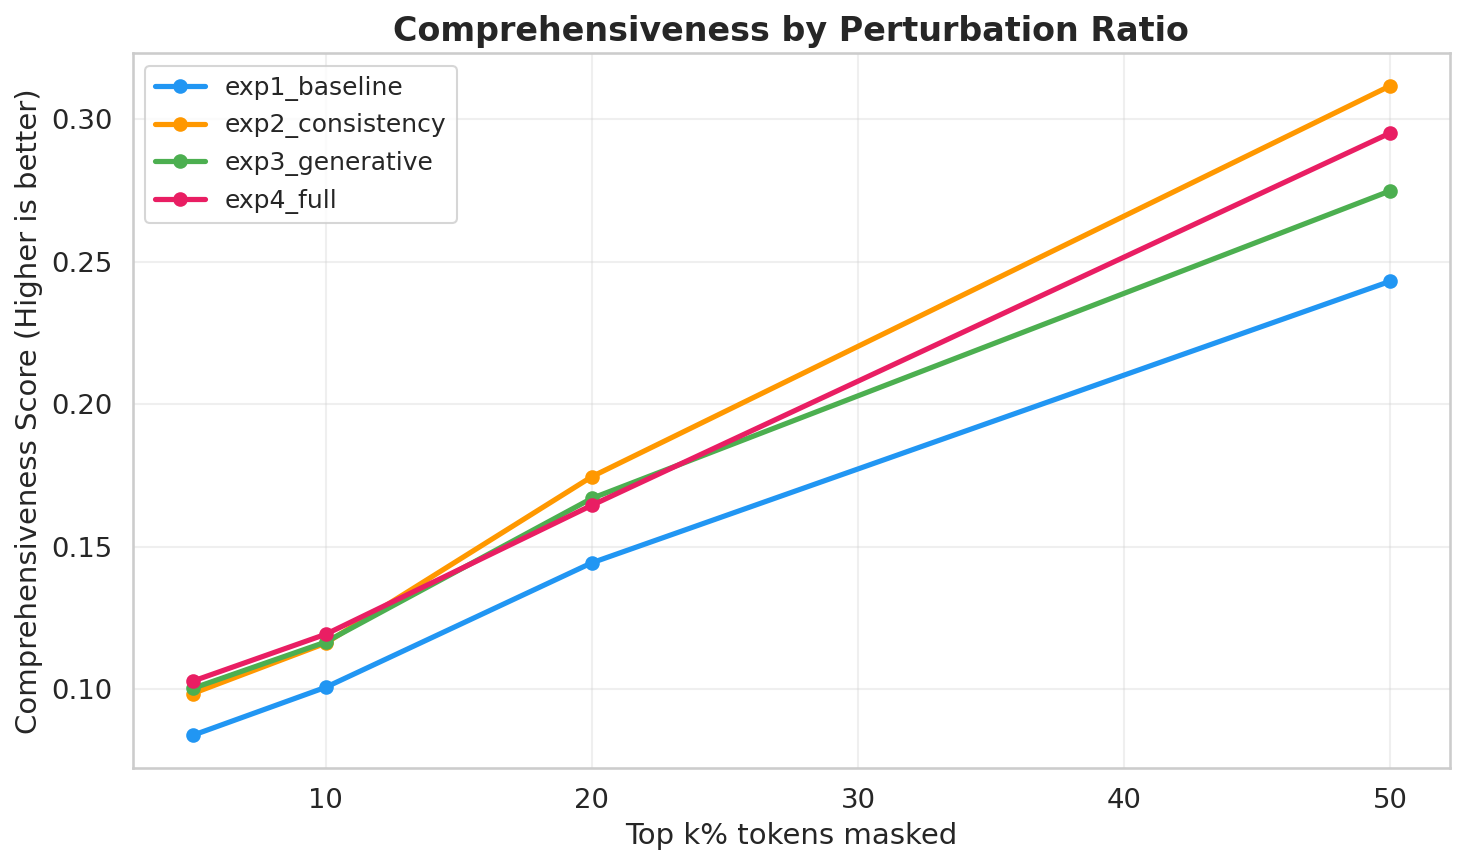
\includegraphics[width=0.88\textwidth]{figures/fig4_confusion_matrices.png}}
\caption{Normalized confusion matrices across Hate Type, Target, and Severity tasks on the 3,553 held-out test set under the proposed full architecture (exp4).}
\label{fig:confusion}
\end{figure*}

\begin{table*}[t]
\caption{Comprehensive Head-to-Head Benchmark on Identical 3,553 Test Set Comparing Our 110M Model with Dedicated Bengali LLMs}
\label{tab:llm_benchmark}
\begin{center}
\resizebox{\textwidth}{!}{
\begin{tabular}{llcccccccc}
\toprule
\textbf{Model} & \textbf{Paradigm} & \textbf{Parameters} & \textbf{Type F1} & \textbf{Target F1} & \textbf{Severity F1} & \textbf{Avg Macro F1} & \textbf{CVR (\%)} & \textbf{Parse Rate} & \textbf{Latency} \\
\midrule
TigerLLM-1B-it \cite{nishat2025tigerllm, raihan2025tigerllm} & 0-shot & 1B & 0.2256 & 0.1851 & 0.3557 & 0.2554 & 0.42\% & 95.6\% & 4.634s \\
TigerLLM-1B-it \cite{nishat2025tigerllm, raihan2025tigerllm} & 5-shot & 1B & 0.3572 & 0.2591 & 0.3747 & 0.3303 & 1.32\% & 99.1\% & 5.851s \\
TituLLM-1B \cite{hishab2024titullm} & 0-shot & 1B & 0.1439 & 0.1500 & 0.2631 & 0.1856 & 0.00\% & 5.7\% & 2.173s \\
TituLLM-1B \cite{hishab2024titullm} & 5-shot & 1B & 0.1803 & 0.1731 & 0.3014 & 0.2183 & 4.98\% & 21.5\% & 5.274s \\
BongLLaMA-3B \cite{banglallm2024bongllama} & 0-shot & 3B & 0.1439 & 0.1500 & 0.2631 & 0.1856 & 0.00\% & 0.0\%* & 0.218s \\
BongLLaMA-3B \cite{banglallm2024bongllama} & 5-shot & 3B & 0.1439 & 0.1500 & 0.0844 & 0.1261 & 100.00\% & 100.0\% & 1.277s \\
\midrule
\textbf{Ours (exp4, Full Model)} & Deterministic & \textbf{110M} & \textbf{0.4994} & \textbf{0.5598} & \textbf{0.6136} & \textbf{0.5576} & \textbf{0.03\%} & \textbf{100.0\%} & \textbf{0.0152s} \\
\bottomrule
\end{tabular}
}
\end{center}
\vspace{-2mm}
{\footnotesize *Note: BongLLaMA 0-shot failed to generate valid JSON, falling back to default majority predictions.}
\end{table*}

\subsection{Comparison with Bengali Large Language Models}
Table \ref{tab:llm_benchmark} presents the master benchmark comparing our 110M model against open-source Bengali LLMs on the identical 3,553 test samples. Fig.~\ref{fig:confusion} visualizes the multi-task confusion matrices for our full model across all three tasks.

\subsubsection{Accuracy Dominance (+68.8\% F1)}
Our 110M model outperforms the strongest Bengali LLM baseline (TigerLLM-1B 5-shot) by +68.8\% relative Macro F1 (0.5576 vs. 0.3303). The LLMs struggle severely with minority classes (such as Gender Hate and Religious Hate), where in-context prompting fails to provide sufficient gradient signal compared to our Focal Loss objective.

\subsubsection{Throughput \& Practical Deployment ($\approx$390$\times$ Faster)}
Our model classifies comments at 0.0152 seconds per sample ($\approx 66$ samples/sec on a single GPU). In contrast, TigerLLM requires 5.851 seconds per sample ($\approx 0.17$ samples/sec $\implies$ $\approx$390$\times$ slower). In large-scale social media streams processing millions of daily comments, deploying 1B--3B LLMs is computationally prohibitive, whereas our 110M architecture can run efficiently on commodity CPUs.

\subsubsection{Syntax Reliability \& Parse Failure Rates}
Our classification heads provide a 100\% deterministic parse rate. Conversely, LLMs exhibit severe parsing fragility: zero-shot BongLLaMA failed completely (0.0\% parse rate), while TituLLM parsed only 5.7\% of zero-shot responses and 21.5\% of 5-shot responses, frequently outputting unstructured natural language that crashes automated moderation software.

\subsubsection{Mode Collapse and BongLLaMA's 100\% CVR}
A profound finding in Table \ref{tab:llm_benchmark} is BongLLaMA-3B's 5-shot collapse (100.00\% CVR). Under in-context learning, BongLLaMA learned the JSON syntax (100\% parse rate) but suffered from \textbf{catastrophic mode collapse}: for all 3,553 test comments, it generated the exact same contradictory string:
\begin{verbatim}
{"type_of_hate": "None", 
 "target_of_hate": "None", 
 "severity_of_hate": "Severe"}
\end{verbatim}
Predicting Type=None while simultaneously asserting Severity=Severe contradicts the taxonomy rule, resulting in 3,553 / 3,553 violations. This provides empirical proof that parameter scale alone (3 Billion parameters) does not prevent logical contradictions; explicit structural constraints are essential.

\subsection{Faithfulness Evaluation (ERASER)}
To evaluate whether the model's explanations faithfully reflect its internal decision-making, we implemented the ERASER framework \cite{deyoung2020eraser} across 1,000 test samples. Attention rationales were extracted from the encoder's [CLS] token and evaluated across token perturbation thresholds $k \in \{5\%, 10\%, 20\%, 50\%\}$.

\begin{table}[t]
\caption{ERASER Faithfulness Metrics on Test Set}
\label{tab:eraser}
\begin{center}
\resizebox{\columnwidth}{!}{
\begin{tabular}{lccc}
\toprule
\textbf{System} & \textbf{Comp.@20\%} & \textbf{Suff.@50\%} & \textbf{AOPC} \\
\midrule
exp1 (Baseline MTL) & 0.144 & 0.099 & 0.143 \\
exp3 (+Gen Head) & 0.167 & 0.106 & 0.165 \\
exp2 (+Consistency Loss) & \textbf{0.175} & 0.117 & \textbf{0.175} \\
exp4 (Full Model) & 0.165 & \textbf{0.075} & 0.170 \\
\bottomrule
\end{tabular}
}
\end{center}
\end{table}

\begin{figure}[t]
\centerline{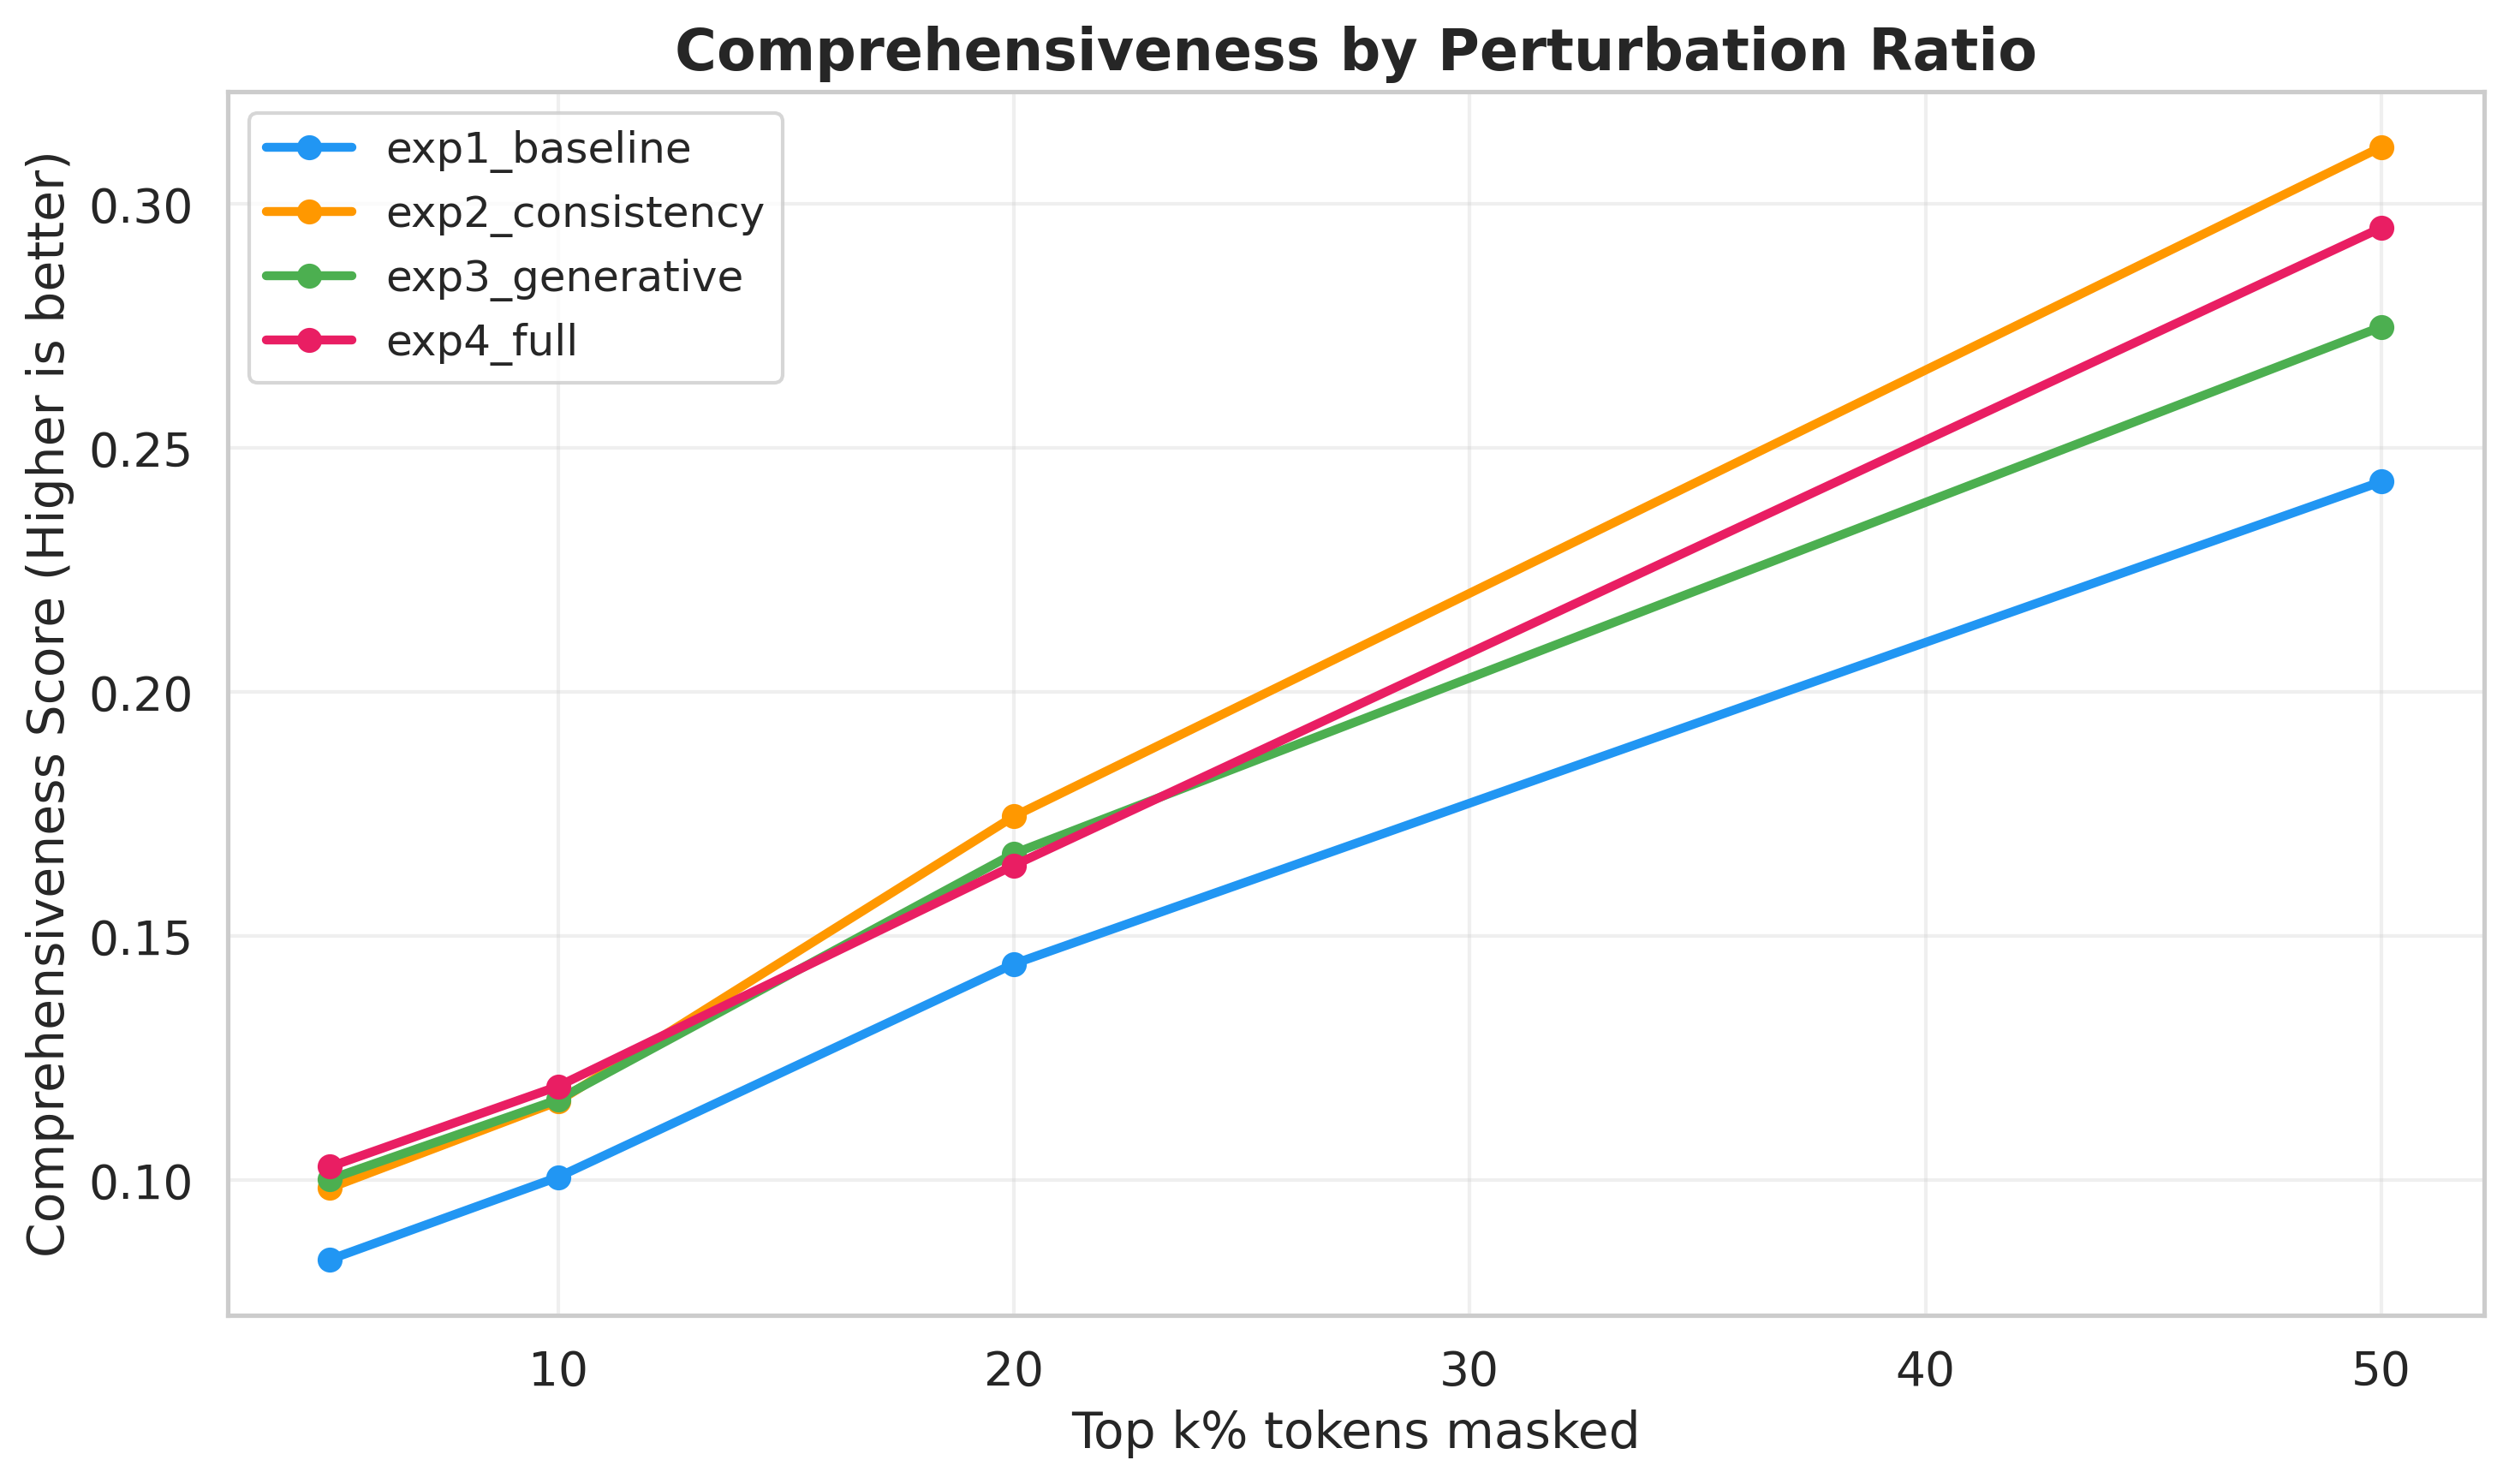
\includegraphics[width=0.92\columnwidth]{figures/fig5_perturbation_curve.png}}
\caption{ERASER Comprehensiveness across token perturbation ratios (5\%, 10\%, 20\%, 50\%). Consistency-constrained models produce consistently more faithful rationales than the unconstrained baseline.}
\label{fig:perturbation}
\end{figure}

As shown in Table \ref{tab:eraser} and Fig.~\ref{fig:perturbation}, models trained with Consistency Loss demonstrate a +22.6\% relative gain in AOPC (0.143 $\rightarrow$ 0.175), proving that structural consistency sharpens internal attention representations. Furthermore, exp4 achieves the lowest Sufficiency score (0.075), confirming that the model's decisions are tightly coupled to the identified rationale tokens.

\subsection{Qualitative Analysis: Dual-Layer Explainability}
Table \ref{tab:qualitative} illustrates our model's dual-layer explainability on representative Bengali test comments. For toxic inputs, the model accurately predicts the full multi-aspect tuple, extracts toxic trigger tokens, and outputs an explanatory justification. For neutral text, the Soft Consistency Loss guarantees that no spurious target or severity is assigned.

\begin{table*}[t]
\caption{Qualitative Examples Illustrating Dual-Layer Explainability}
\label{tab:qualitative}
\begin{center}
\resizebox{\textwidth}{!}{
\begin{tabular}{p{4.8cm}p{3.2cm}p{3.2cm}p{5.5cm}}
\toprule
\textbf{Input Bengali Comment} & \textbf{Predicted Tuple} & \textbf{Extracted Rationale} & \textbf{Generated Explanation (Bengali)} \\
\midrule
\textit{``সরকারের উচিত বাংলাদেশেও মন্দির ভেঙে মসজিদ করা''} & Type: Religious Hate \newline Target: Community \newline Severity: Severe & \textit{[মন্দির ভেঙে, মসজিদ করা]} & এই মন্তব্যটিতে একটি নির্দিষ্ট ধর্মীয় সম্প্রদায়ের উপাসনালয় ধ্বংসের সহিংস আহ্বান জানানো হয়েছে, যা সরাসরি ধর্মীয় বিদ্বেষ সৃষ্টি করে। \\
\midrule
\textit{``মেসি বোলে কথা মেসি মেসি মেসি এবং মেসি কিছু বলতে হবে না''} & Type: None \newline Target: None \newline Severity: Little to None & \textit{[খেলাধুলা, প্রশংসা]} & মন্তব্যটি ক্রীড়া বিষয়ক এবং একজন খেলোয়াড়ের প্রতি সাধারণ প্রশংসাসূচক অভিব্যক্তি, এতে কোনো বিদ্বেষপূর্ণ উপাদান নেই। \\
\bottomrule
\end{tabular}
}
\end{center}
\end{table*}

\section{Conclusion}
We presented a Consistency-Constrained Multi-Task Learning framework for multi-aspect Bengali hate speech detection. By introducing a differentiable Soft Consistency Loss, our model eliminates 99.7\% of logical contradictions on held-out test data while boosting Average Macro F1 to 0.558. In head-to-head benchmarking, our 110M model outperforms 1B--3B open-source Bengali LLMs by +68.8\% in Macro F1 while running $\approx$390$\times$ faster with 100\% deterministic parsing. Furthermore, integrated rationale distillation produces faithful natural language explanations validated via ERASER metrics. These findings prove that task-specific structural inductive biases are far more effective, reliable, and cost-efficient than raw parameter scale for automated content moderation in low-resource languages.

\section*{Acknowledgment}
The authors acknowledge the high-performance computing resources provided for training and evaluating the models in this research.

\bibliographystyle{IEEEtran}
\bibliography{references}

\end{document}
